\section{Systematic Uncertainties} \label{sec:sys}
The systematic uncertainties on the \gagg\ limits arise from the 
following sources:
\begin{itemize}
\item Uncertainty on the product 
$\left.Q_L\beta\middle/\left(1+\beta\right)\right.$ in Eq.~\eqref{eq:ps}: 
In order to extract the loaded quality factor $Q_L$ and the coupling 
coefficient $\beta$, a fitting of the measured results of the cavity 
scattering matrix was performed. A relative uncertainty of 3.6\% is 
assigned to this product, after a comparison of the measurements at 
$T_\text{c}\simeq155$~mK with a prediction extrapolated from the measurements 
at room temperature. More details about the measurements of the 
cavity properties can be found in Ref.~\cite{TASEHInstrumentation}. 
A 3.6\% variation of this product results in a 1.9\% uncertainty 
on the \gagg\ limits. 

\item Uncertainties on the noise temperature \ta\ from: (i) the RMS of 
the measurements in the calibration: 
$\left. \Delta \ta\middle/\ta\right.= 2.3\%$,  
%(see Sec.~\ref{sec:calibration} and Fig.~\ref{fig:hemtcalvsf}).
%
%\item Uncertainty on the noise temperature \ta\ 
and (ii) from the largest difference 
between the value determined by the calibration and that from the CD102 
data: $\left. \Delta \ta\middle/\ta\right.= 4\%$ 
(see Sec.~\ref{sec:calibration} and Fig.~\ref{fig:hemtcalvsf}). 
These two uncertainties on the \ta\ result in a 2.8\% uncertainty 
on the \gagg\ limits. 

%\item Uncertainty on the misalignment $\delta f_m$ between the true 
%axion frequency $f_a$ and the lower bin boundaries in the merged spectrum 
%(see Sec.~\ref{sec:merge}).
\item Uncertainty due to the misalignment (see Sec.~\ref{sec:merge}):
  estimated by comparing the central results to the one without misalignment
  ($\delta f_m = 0$)
  and to the ones with given values of $\delta f_m$.
  The comparison shows that $\delta f_m = 0$ gives the largest difference 
  of 2.8\% on the limit, which is used as the systematic uncertainy from the 
  misalignment.
  
\item Uncertainty from the choice of the SG-filter parameters: i.e.  
the window width and the order of the polynomial in the SG filter. At the 
beginning of the data taking, a preliminary optimization was performed: a 
window width of 201 bins and a 4$^\text{th}$-order polynomial were used for 
the first analysis of the CD102 data (see Sec.~\ref{sec:ana}). 
This choice is kept for the central results. 
Nevertheless, various methods of optimization are also explored. The goal 
of the optimization is to find a set of SG-filter parameters that only 
model the noise spectrum and do not remove a real signal. 
The methods include:
\begin{itemize}
 \item Minimize the difference between the two outputs returned by the SG 
filter, when the SG filter is applied to: (i) the real data only, and (ii) 
the sum of the real data and the simulated axion signals. 
 \item Minimize the difference between the output returned by the 
 SG filter and the function ${\cal G}_\text{noise}$ 
that models the noise spectrum (derived by fitting the CD102 data), 
when the SG filter is applied to the sum of the simulated noise based on 
${\cal G}_\text{noise}$ and the simulated axion signals. 
See Fig.~\ref{fig:sgcompare} for an example of the 
simulated spectrum, the function ${\cal G}_\text{noise}$, and the 
output returned by 
 the SG filter when a 3$^\text{rd}$-order polynomial and a window of 141 
 bins are chosen; the differences from all the frequency bins are summed 
 together when performing the optimization.
 Figure~\ref{fig:sgoptimize} shows the difference 
as a function of window widths when the order of polynomial is 
 set to three, four, and six. 
 \item Compare the mean $\mu_\text{noise}$ and the width $\sigma_\text{noise}$ 
of the measured power after applying the SG filter, 
assuming that no signal is present in the 
data. See Fig.~\ref{fig:noisegauss} for an example distribution 
of the measured power from the averaged spectrum of a 
single scan; %, when the cavity resonant frequency 
%is 4.798147~GHz; 
a Gaussian fit is performed to extract 
$\mu_\text{noise}$ and $\sigma_\text{noise}$. Given the nature of the 
thermal noise, the two variables are supposed to be related to 
each other if proper window width and order are chosen:
\begin{equation*} 
\sigma_\text{noise} = \frac{\mu_\text{noise}}{\sqrt{N_\text{spectra}}},
\end{equation*}
where $N_\text{spectra}$ is the number of spectra for averaging and 
is related to the amount of integration time for each frequency step. In 
general, $N_\text{spectra}=1920000-2520000$. 
\end{itemize}

In addition, one could choose to optimize for each frequency step 
individually, optimize for a certain frequency step but apply the results to 
all data, or optimize by adding all the frequency steps together. 
%Figure~\ref{fig:syssgfilter} shows that 
The deviations from the central results using different optimization 
approaches are in general within 1\% and the 
maximum deviation of 1.8\% 
on the \gagg\ limit is used as a conservative estimate of the systematic 
uncertainty from the SG filter. 

\end{itemize}

%The first source of the systematic uncertainty 
%has negligible effect on the limits of \gagg\ while the 
%latter three sources are studied and added in quadrature to obtain the total 
%systematic uncertainty. 
The effects on the \gagg\ limits from these sources are studied and added in 
quadrature to obtain the total systematic uncertainty. 
The systematic uncertainties on the \gagg\ limits 
are displayed together with the central results in Sec.~\ref{sec:results}. 
%Overall the total relative systematic uncertainty is $\approx 3.4\%$.
Overall the total relative systematic uncertainty is $\approx 4.6\%$.

\begin{figure} [htbp]
  \centering
  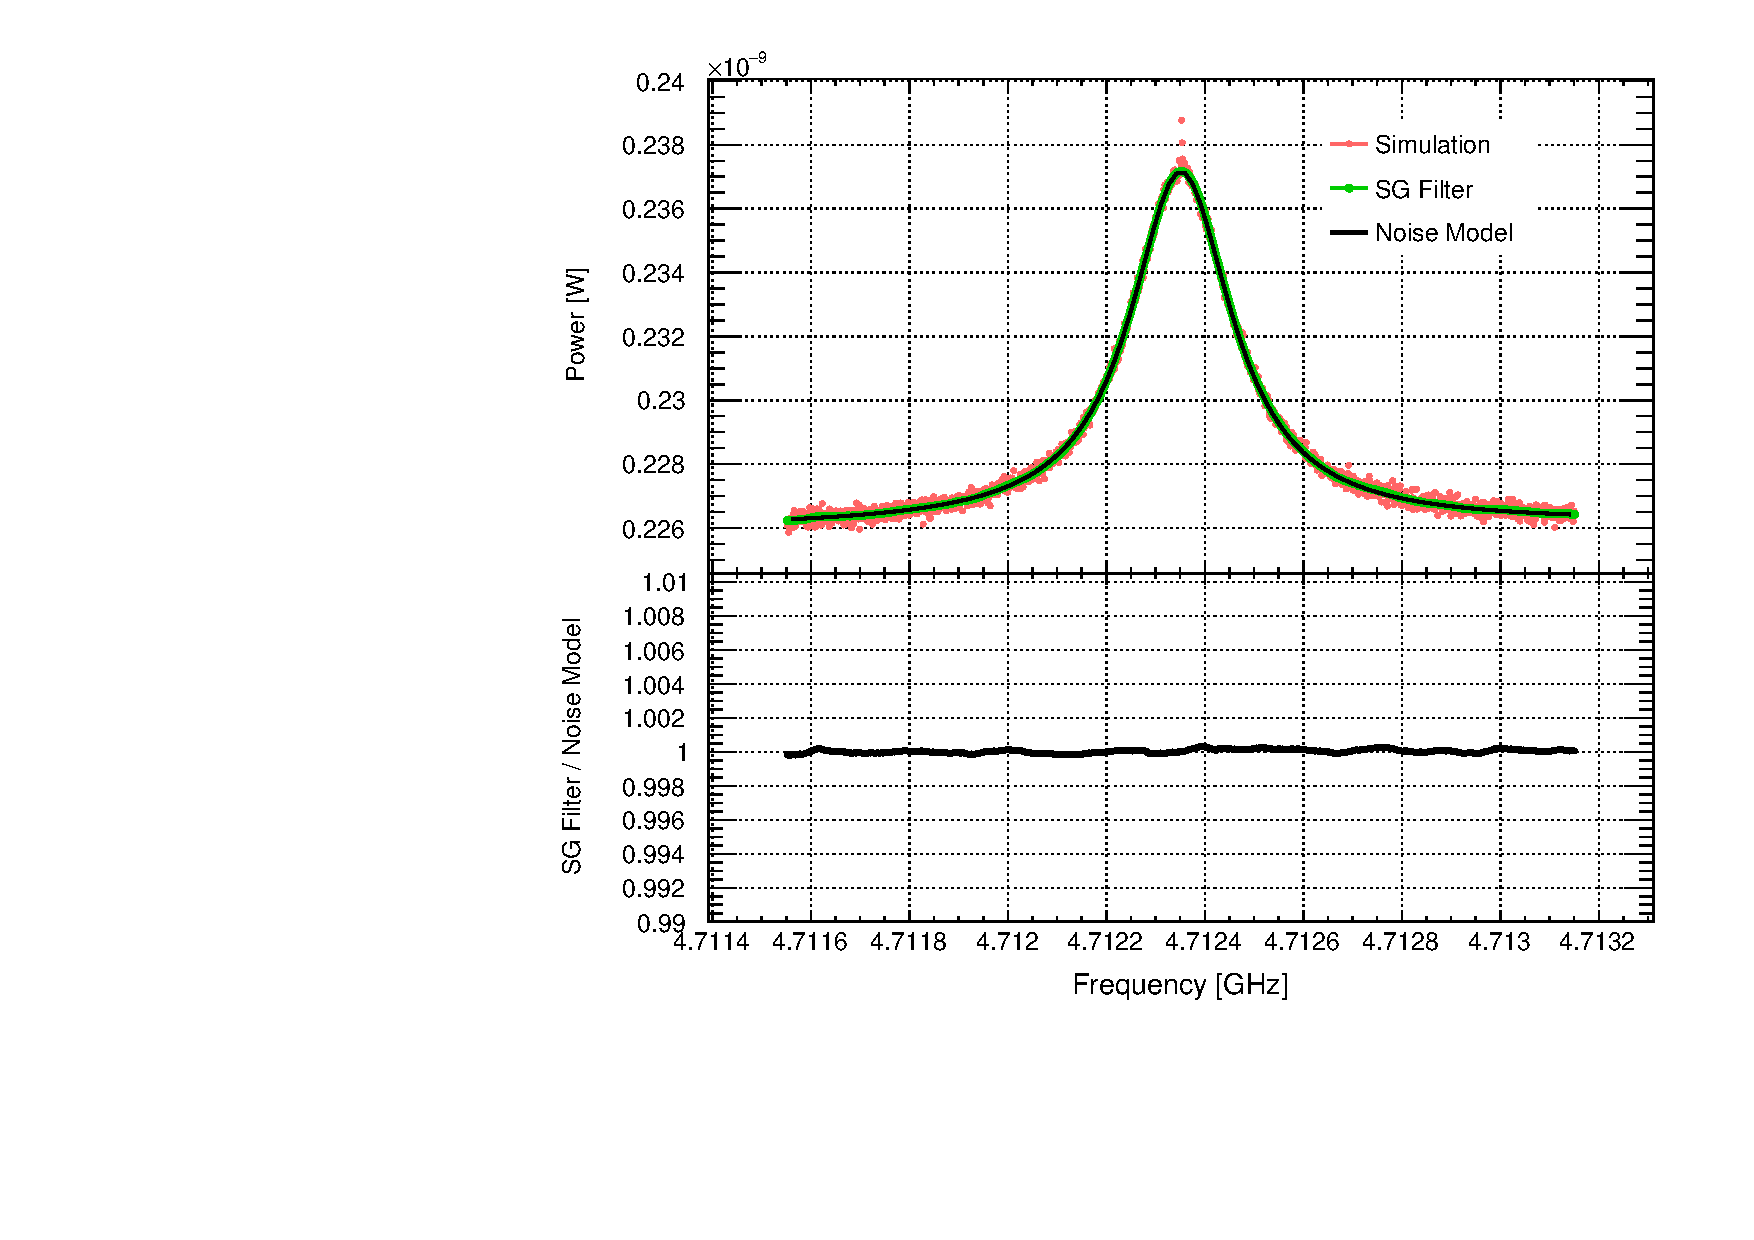
\includegraphics[width=8.6cm]{figures/GeneratedSpectrum_Optimized_SGFilter_NPar_3_Window_141.pdf}
  \caption{Upper panel: 
 The simulated spectrum (red), including the axion signal and the 
noise, is overlaid with the function that models the noise 
${\cal G}_\text{noise}$ (black) and the 
output returned by the SG filter (green). Lower panel: The ratio of the output 
returned by the SG filter to the function ${\cal G}_\text{noise}$.}
  \label{fig:sgcompare}
\end{figure}


\begin{figure} [htbp]
  \centering
%  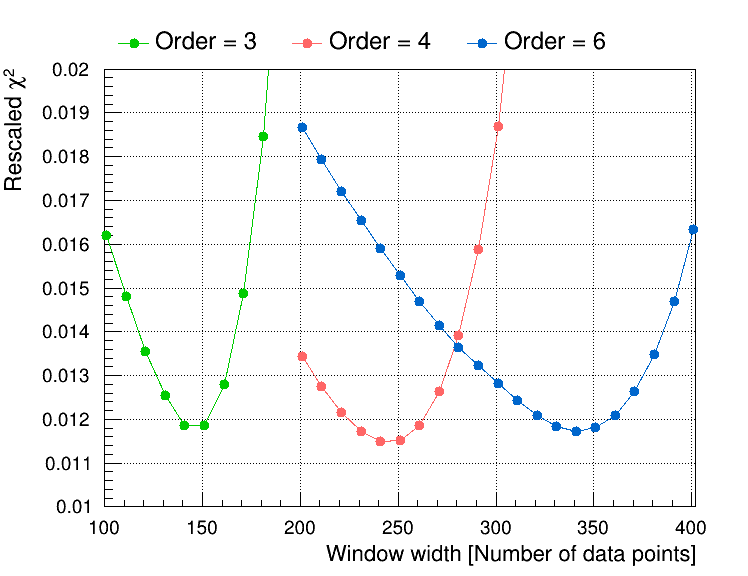
\includegraphics[width=0.4\textwidth,height = 0.25\textwidth]{figures/chi2_Different_Order_Window_SGFilter.png}
  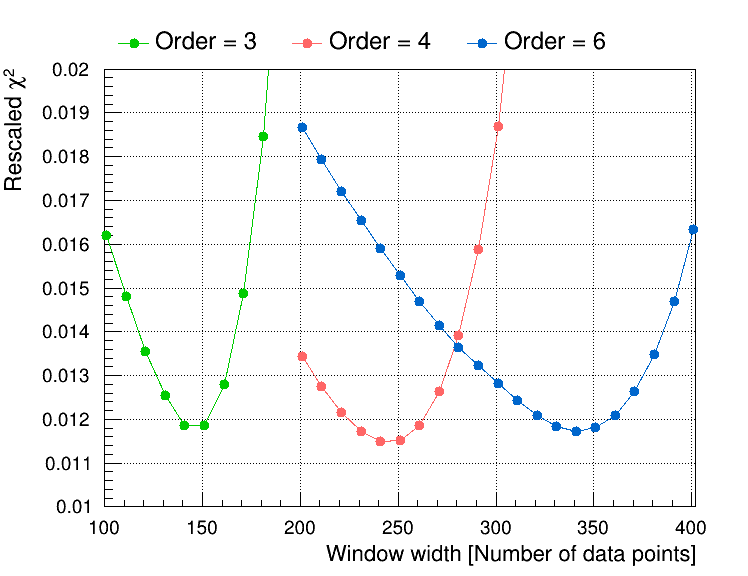
\includegraphics[width=8.6cm]{figures/chi2_Different_Order_Window_SGFilter.png}
  \caption{The difference between the output returned by the SG filter 
  and the function that models the noise spectrum, when various values of 
  window widths and 
  a 3$^\text{rd}$, a 4$^\text{th}$, or a 
  6$^\text{th}$-order polynomial are applied in the SG filter. In this 
  figure, the best choice is a 4$^\text{th}$-order polynomial with 
  a window width of 241 data points (bins). }
  \label{fig:sgoptimize}
\end{figure}
 


\begin{figure} [htbp]
  \centering
  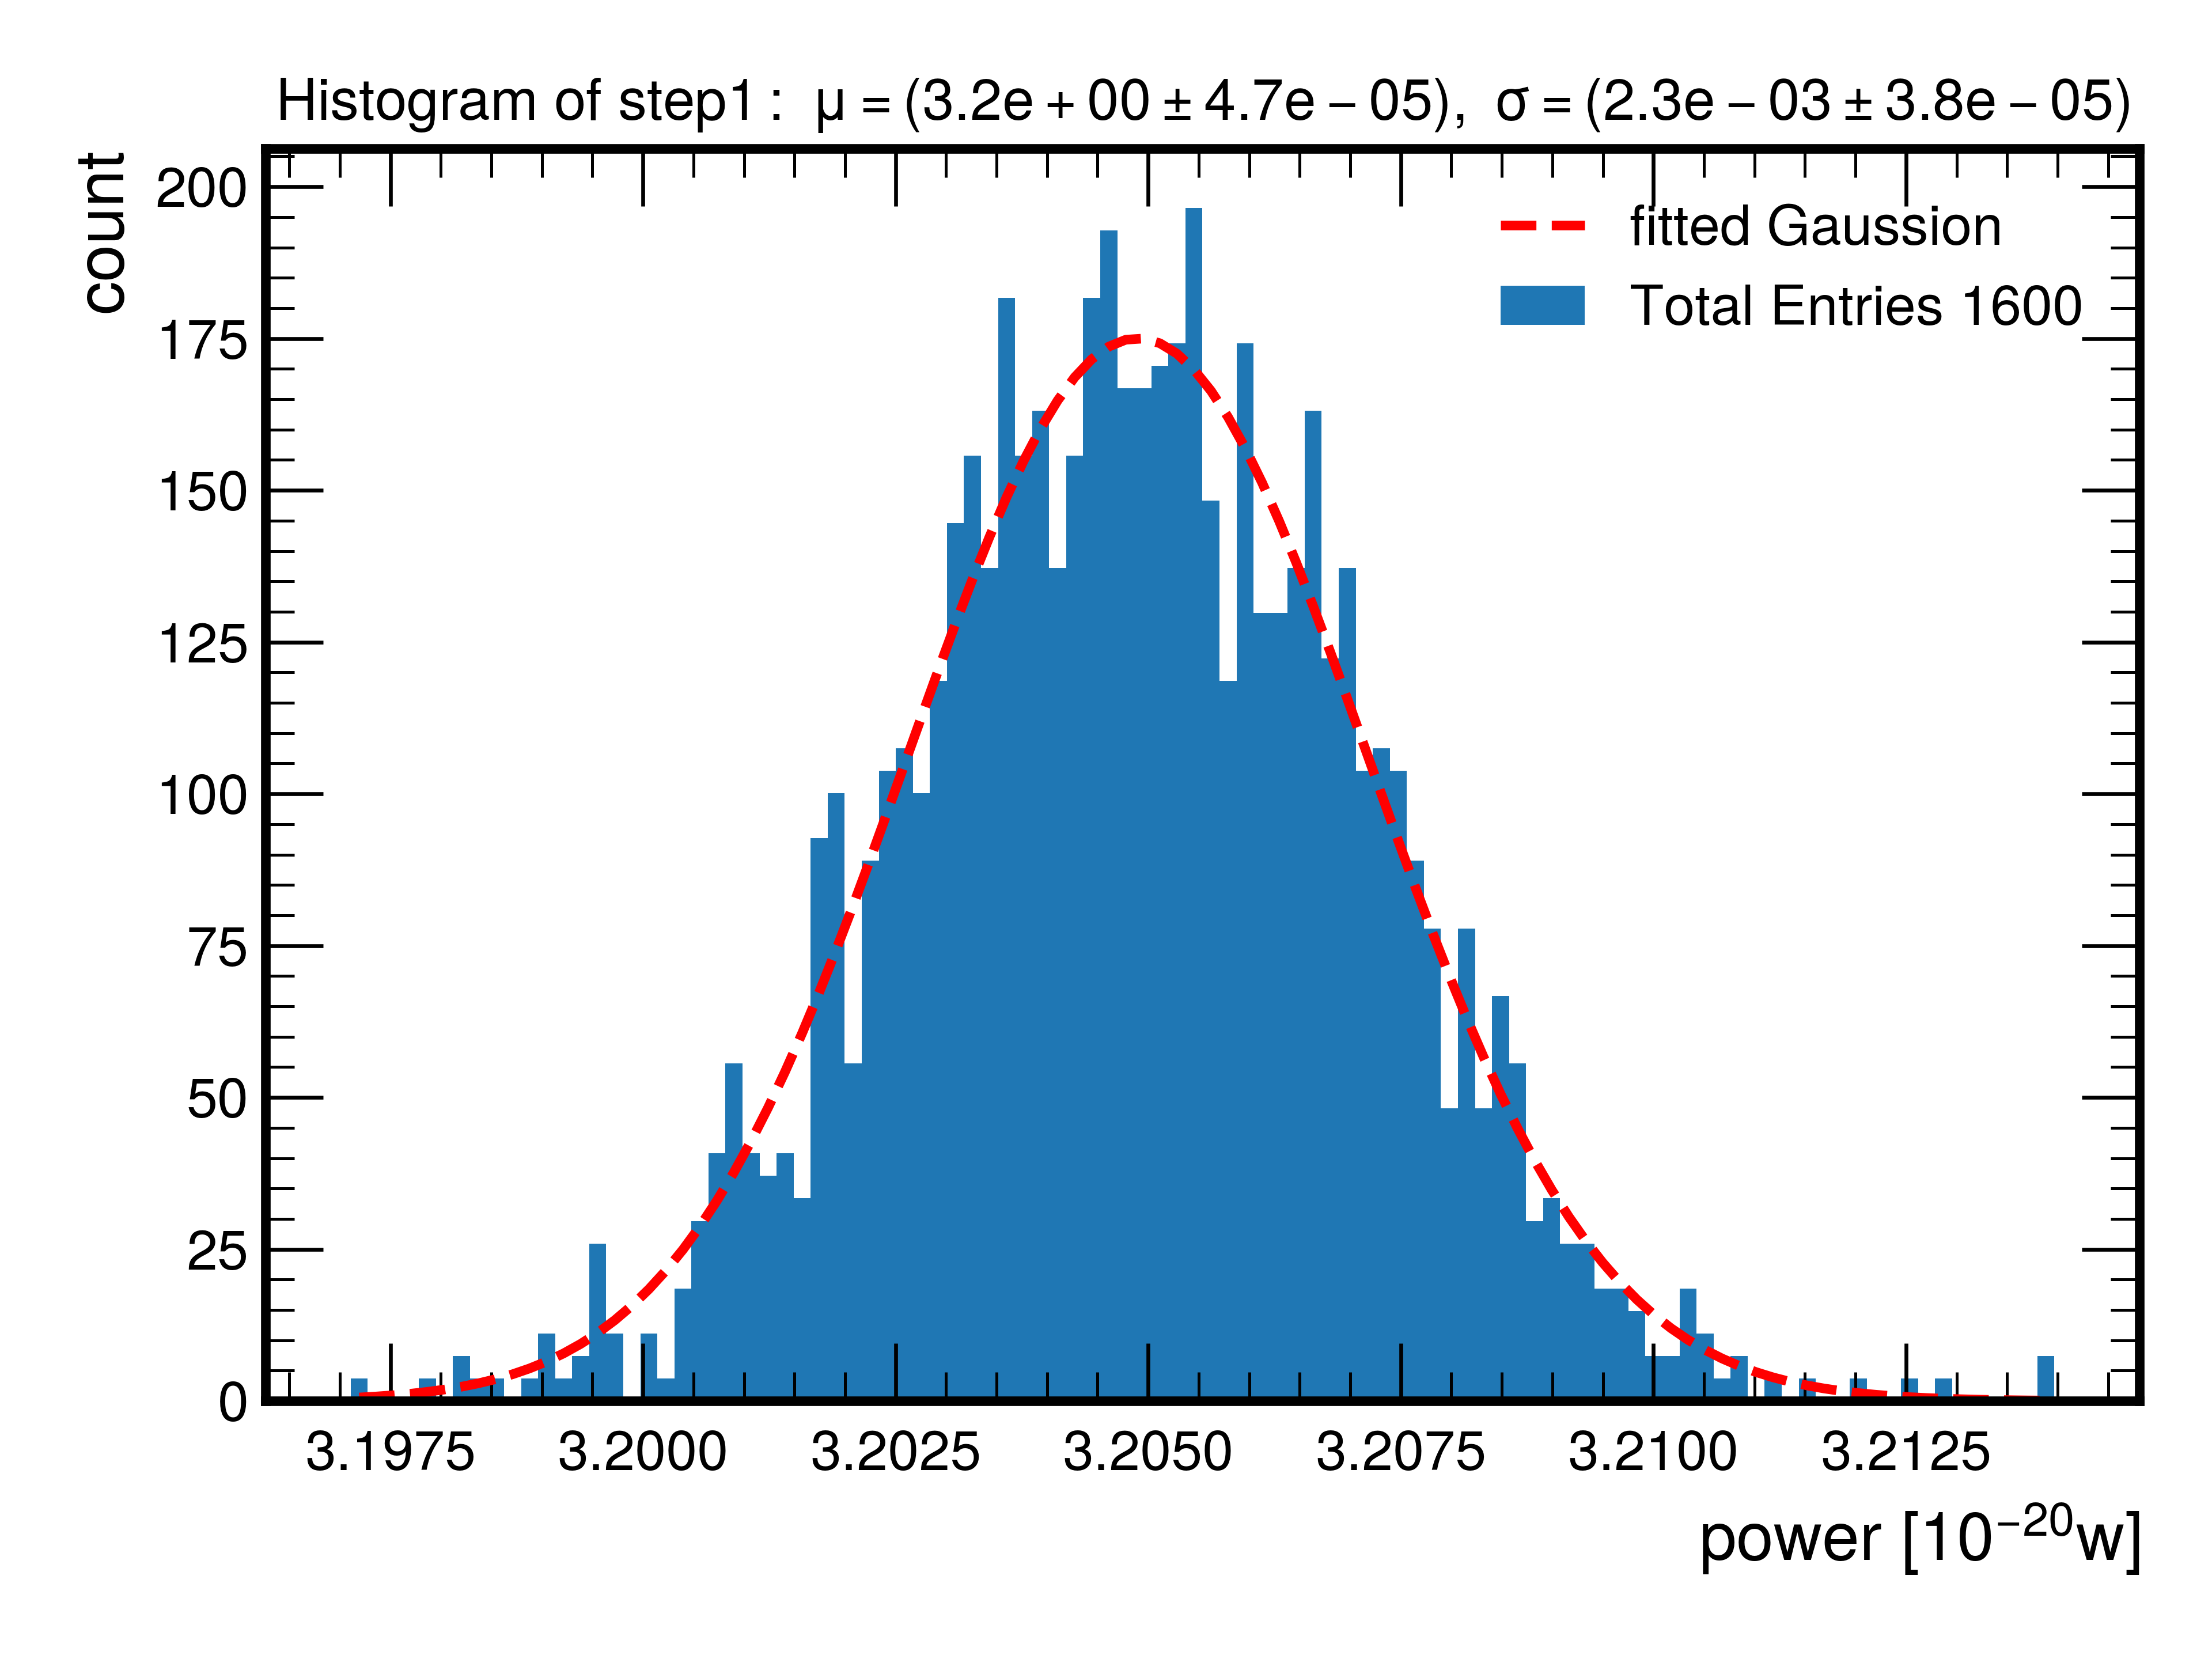
\includegraphics[width=8.6cm]{figures/sysSG_temphistogram.png}
  \caption{An example of the distribution of the measured power after 
applying the SG filter, when 
the cavity resonant frequency is 4.798147~GHz. The distribution contains 
1600 entries and each entry corresponds to the measured power 
in one frequency bin, averaged
over 1920000 subspectra. The mean and the width returned by 
a Gaussian fit to the distribution are used to determine the best choice of 
SG parameters. The fitted Gaussian mean $\mu$ divided by 
$\sqrt{1920000}$ is consistent 
with the fitted Gaussian width $\sigma$. The best choice of SG parameters 
obtained for this scan is a window of 189 data points (bins) with a 
3$^\text{rd}$-order polynomial. 
%The mean $\mu_\text{noise}=3.2\times10^{-20}$~W in 
%a 1-kHz frequency bin would imply a noise temperature of 2.3~K.
}
  \label{fig:noisegauss}
\end{figure}
 

%\begin{figure} [htbp]
%  \centering
%  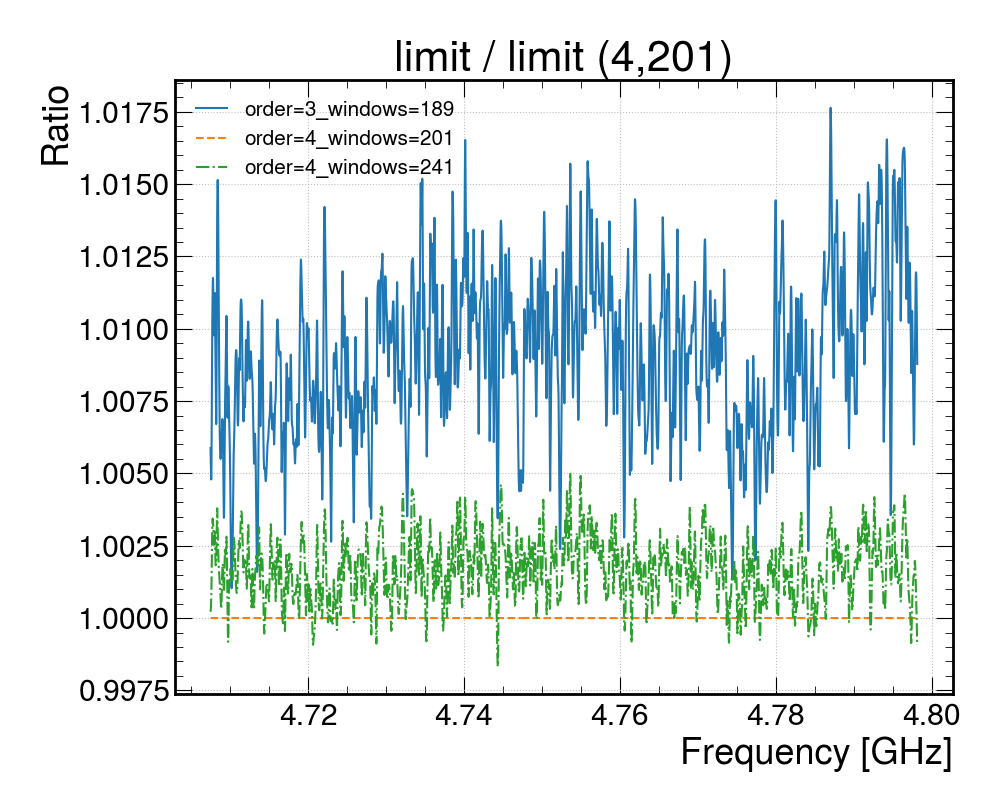
\includegraphics[width=8.6cm]{figures/sys_compareSG_4_201.png}
%  \caption{The ratios of the limits on \gagg\ due to the different choices 
% of the window width and the order of polynomial in the SG filter, with 
%respect to 
% the central results (a window width of 201 bins and the 4$^\text{th}$-order 
% polynomial). The window width of 241 bins and the 4$^\text{th}$-order 
% polynomial are obtained from the optimization after injecting an axion 
%signal on top of a simulated noise spectrum. The window width of 189 bins and 
%the 3$^\text{rd}$-order polynomial are obtained from the optimization 
% after comparing the means and the widths of the measured power distributions.}
%  \label{fig:syssgfilter}
%\end{figure}
 

